\documentclass[11pt]{article}
\usepackage{theme}
\usepackage{shortcuts}
% Document parameters
% Document title
\title{Assignment 3 (ML for TS) - MVA}
\author{
Léa Bohbot \email{lea.bohbot@polytechnique.edu} \\ % student 1
Grégoire Béchade \email{gregoire.bechade@gmail.com} % student 2
}

\begin{document}
\maketitle

\section{Introduction}

\paragraph{Objective.} The goal is to implement (i) a signal processing pipeline with a change-point detection method and (ii) wavelets for graph signals.

\paragraph{Warning and advice.} 
\begin{itemize}
    \item Use code from the tutorials as well as from other sources. Do not code yourself well-known procedures (e.g. cross validation or k-means), use an existing implementation.
    \item The associated notebook contains some hints and several helper functions.
    \item Be concise. Answers are not expected to be longer than a few sentences (omitting calculations).
\end{itemize}



\paragraph{Instructions.}
\begin{itemize}
    \item Fill in your names and emails at the top of the document.
    \item Hand in one report per pair of students.
    \item Rename your report and notebook as follows:\\ \texttt{FirstnameLastname1\_FirstnameLastname1.pdf} and\\ \texttt{FirstnameLastname2\_FirstnameLastname2.ipynb}.\\
    For instance, \texttt{LaurentOudre\_CharlesTruong.pdf}.
    \item Upload your report (PDF file) and notebook (IPYNB file) using the link given in the email.
\end{itemize}

% ------------------------------------------------------------------------------
\newpage
\section{Dual-tone multi-frequency signaling (DTMF)}

\href{https://en.wikipedia.org/wiki/Dual-tone\_multi-frequency\_signaling}{Dual-tone multi-frequency signaling} is a procedure to encode symbols using an audio signal.
The possible symbols are 0, 1, 2, 3, 4, 5, 6, 7, 8, 9, *, \#, A, B, C, and D.
A symbol is represented by a sum of cosine waves: for $t=0,1,\dots, T-1$,

$$
y_t = \cos(2\pi f_1 t/f_s) + \cos(2\pi f_2 t/f_s)
$$
where each combination of $(f_1, f_2)$ represents a symbols.
The first frequency has four different levels (low frequencies), and the second frequency has four other levels (high frequencies); there are 16 possible combinations.
In the notebook, you can find an example symbol sequence encoded with sound and corrupted by noise (white noise and a distorted sound).

\begin{exercise}
Design a procedure that takes a sound signal as input and outputs the sequence of symbols. 
To that end, you can use the provided training set.
The signals have a varying number of symbols with a varying duration. 
There is a brief silence between each symbol.

Describe in 5 to 10 lines your methodology and the calibration procedure (give the hyperparameter values). Hint: use the time-frequency representation of the signals, apply a change-point detection algorithm to find the starts and ends of the symbols and silences, and then classify each segment. 

\end{exercise}
\begin{solution}
    The methodology we used was the following: 
    We plotted spectrograms of the signals to observe that the signal were characterized by two frequencies band aligned. 
    There were also a time-varying frequency band that we wanted avoid. 
    We decided to detect the 3 most important frequencies at each time step and sort them by increasing order. 
    We then averaged them to have the "mean most important frequency". 
    A Dynp algo was then launched on this time series to detect the change points, with the indication of the number of changed points obtained thanks to the length of the symbol sequence. 
    For each portion detected in the signal, we found the two fundamental frequencies as the max 2 values of the histogram of the 3 maximum frequences recorded during this sequences. 
    This procedure enabled to avoid the noise.
    We the created a dictionary that had as keys the symbols and at values the top and low frequencies of the signals labelled as this symbol.
    Then, the median value of top and low frequencies was taken, to prevent badly detecetd signals to introduce errors. 
    The test sequences were classified as follows: the spectrogram was plotted to determine the length of the sequence. 
    The frequencies were identified as explained above, and the symbol of the subsequence was determined as the closest in the whole dictionary. 

\end{solution}

\begin{exercise}
What are the two symbolic sequences encoded in the test set?
\end{exercise}

\begin{solution}
    \begin{itemize}
        \item Sequence 1: '7', '2', '1', 'C', '9', '9'
        \item Sequence 2: '1', '\#', '2', '\#' 
    \end{itemize}
\end{solution}

% ------------------------------------------------------------------------------
\newpage
\section{Wavelet transform for graph signals}
Let $G$ be a graph defined a set of $n$ nodes $V$ and a set of edges $E$. A specific node is denoted by $v$ and a specific edge, by $e$.
The eigenvalues and eigenvectors of the graph Laplacian $L$ are $\lambda_1\leq\lambda_2\leq\dots\leq \lambda_n$ and $u_1$, $u_2$, \dots, $u_n$ respectively.

For a signal $f\in\RR^{n}$, the Graph Wavelet Transform (GWT) of $f$ is $ W_f: \{1,\dots,M\}\times V \longrightarrow \RR$:
\begin{equation}
    W_f(m, v) := \sum_{l=1}^n \hat{g}_m(\lambda_l)\hat{f}_l u_l(v)
\end{equation}
where $\hat{f}= [\hat{f}_1,\dots,\hat{f}_n]$ is the Fourier transform of $f$ and $\hat{g}_m$ are $M$ kernel functions.
The number $M$ of scales is a user-defined parameter and is set to $M:=9$ in the following.
Several designs are available for the $\hat{g}_m$; here, we use the Spectrum Adapted Graph Wavelets (SAGW).
Formally, each kernel $\hat{g}_m$ is such that
\begin{equation}
    \hat{g}_m(\lambda) := \hat{g}^U(\lambda - am) \quad (0\leq\lambda\leq\lambda_n)
\end{equation}
where $a:=\lambda_n / (M+1-R)$,
\begin{equation}
    \hat{g}^U(\lambda) := \frac{1}{2}\left[ 1 + \cos\left( 2\pi\left(\frac{\lambda}{a R}  + \frac{1}{2} \right)\right) \right]\one(-Ra \leq \lambda < 0)
\end{equation}
and $R>0$ is defined by the user.

\begin{exercise}
Plot the kernel functions $\hat{g}_m$ for $R=1$, $R=3$ and $R=5$ (take $\lambda_n=12$) on Figure~\ref{fig:sagw-kernels}. What is the influence of $R$?
\end{exercise}

\begin{solution}
\begin{figure}
    \centering
    \begin{minipage}[t]{0.32\textwidth}
    \centerline{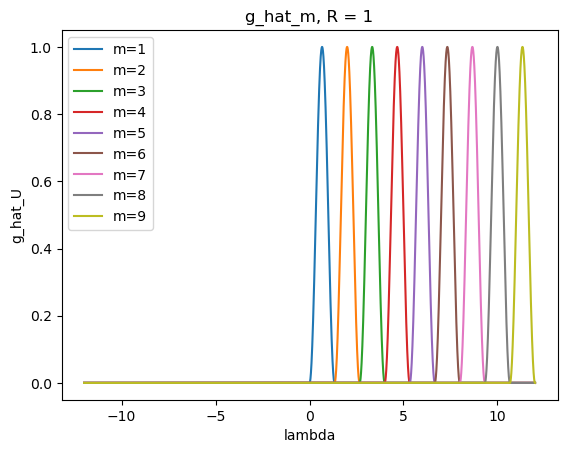
\includegraphics[width=\textwidth]{q3_a.png}}
    \centerline{(a) $R=1$}
    \end{minipage}
    \hfill
    \begin{minipage}[t]{0.32\textwidth}    \centerline{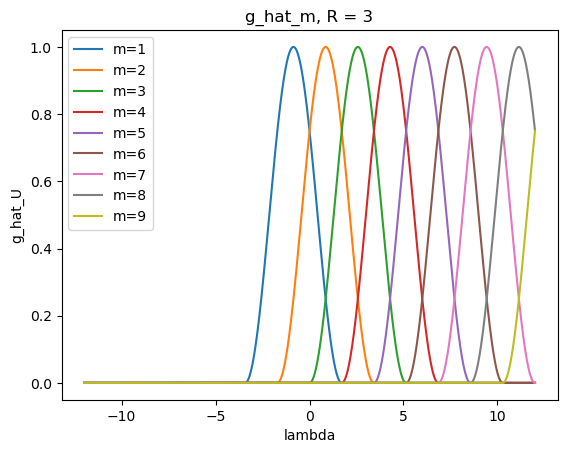
\includegraphics[width=\textwidth]{q3_b.png}}
    \centerline{(b) $R=3$}
    \end{minipage}
    \hfill
    \begin{minipage}[t]{0.32\textwidth}    \centerline{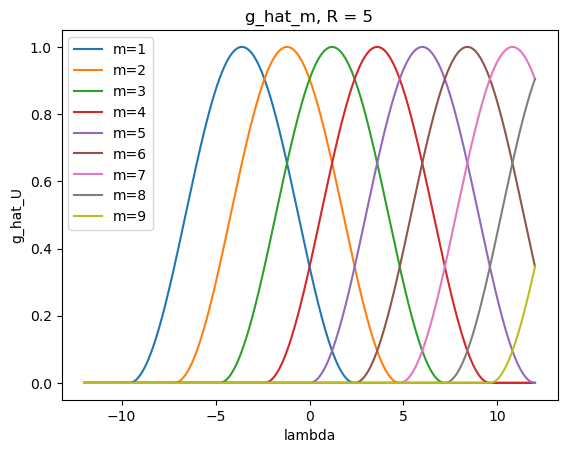
\includegraphics[width=\textwidth]{q3_c.png}}
    \centerline{(c) $R=5$}
    \end{minipage}
    \caption{The SAGW kernels functions}\label{fig:sagw-kernels}
\end{figure}

R increases the variance of the functions and shifts them to the left. 
\end{solution}


\newpage
We will study the Molene data set (the one we used in the last tutorial).
The signal is the temperature.

\begin{exercise}
Construct the graph using the distance matrix and exponential smoothing (use the median heuristics for the bandwidth parameter). 
\begin{itemize}
    \item Remove all stations with missing values in the temperature.
    \item Choose the minimum threshold so that the network is connected and the average degree is at least 3.
    \item What is the time where the signal is the least smooth?
    \item What is the time where the signal is the smoothest?
\end{itemize}
\end{exercise}

\begin{solution}
The stations with missing values are ARZAL, BREST-GUIPAVAS, BRIGNOGAN, LANDIVISIAU, LANNAERO, LANVEOC, OUESSANT-STIFF, QUIMPER, ST NAZAIRE-MONTOIR. 

The threshold is equal to 0.74

The signal is the least smooth at 2014-01-21 02:00:00 (signal not smooth when smoothness is high). 

The signal is the smoothest at 2014-01-24 23:00:00 (signal smooth when smoothness is low).

\end{solution}

\newpage
\begin{exercise}
(For the remainder, set $R=3$ for all wavelet transforms.)

For each node $v$, the vector $[W_f(1, v), W_f(2, v),\dots, W_f(M, v)]$ can be used as a vector of features. We can for instance classify nodes into low/medium/high frequency: 
\begin{itemize}
    \item a node is considered low frequency if the scales $m\in\{1,2,3\}$ contain most of the energy,
    \item a node is considered medium frequency if the scales $m\in\{4,5,6\}$ contain most of the energy,
    \item a node is considered high frequency if the scales $m\in\{6,7,9\}$ contain most of the energy.
\end{itemize}


For both signals from the previous question (smoothest and least smooth) as well as the first available timestamp, apply this procedure and display on the map the result (one colour per class).

\end{exercise}

\begin{solution}
\begin{figure}
    \centering
    \begin{minipage}[t]{0.45\textwidth}
    \centerline{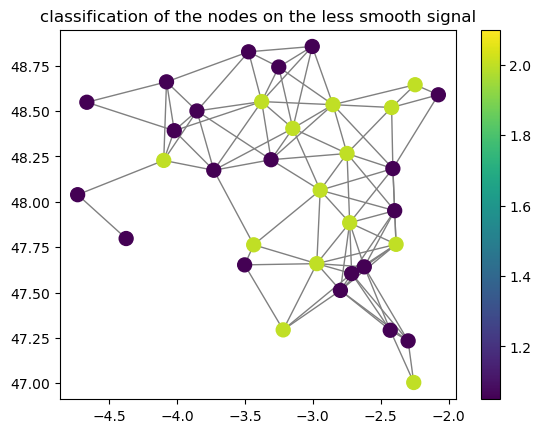
\includegraphics[width=\textwidth]{q5_a.png}}
    \centerline{(a) Least smooth signal}
    \end{minipage}
    \hfill
    \begin{minipage}[t]{0.45\textwidth}    \centerline{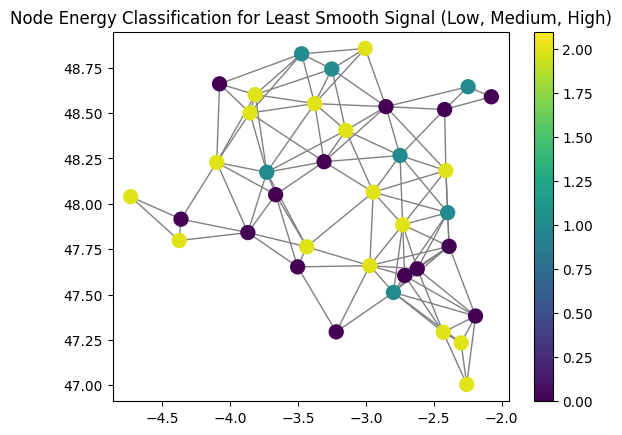
\includegraphics[width=\textwidth]{q5_b.png}}
    \centerline{(b) Smoothest signal}
    \end{minipage}
    \vskip1em
    \begin{minipage}[t]{0.45\textwidth}    \centerline{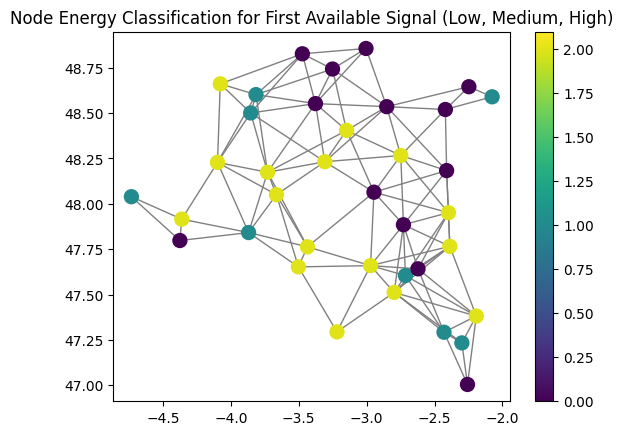
\includegraphics[width=\textwidth]{q5_c.png}}
    \centerline{(c) First available timestamp}
    \end{minipage}
    \caption{Classification of nodes into low/medium/high frequency}\label{fig:node-classif}
\end{figure}
\end{solution}

\newpage
\begin{exercise}
Display the average temperature and for each timestamp, adapt the marker colour to the majority class present in the graph (see notebook for more details).
\end{exercise}

\begin{solution}
\begin{figure}
    \centering
    \begin{minipage}[t]{0.8\textwidth}
    \centerline{\includegraphics[width=\textwidth]{example-image-golden}}
    \end{minipage}
    \caption{Average temperature. Markers' colours depend on the majority class.}
\end{figure}
\end{solution}

\newpage
\begin{exercise}
The previous graph $G$ only uses spatial information.
To take into account the temporal dynamic, we construct a larger graph $H$ as follows: a node is now \textit{a station at a particular time} and is connected to neighbouring stations (with respect to $G$) and to itself at the previous timestamp and the following timestamp.
Notice that the new spatio-temporal graph $H$ is the Cartesian product of the spatial graph $G$ and the temporal graph $G'$ (which is simply a line graph, without loop).

\begin{itemize}
    \item Express the Laplacian of $H$ using the Laplacian of $G$ and $G'$ (use Kronecker products).
    \item Express the eigenvalues and eigenvectors of the Laplacian of $H$ using the eigenvalues and eigenvectors of the Laplacian of $G$ and $G'$.
    \item Compute the wavelet transform of the temperature signal.
    \item Classify nodes into low/medium/high frequency and display the same figure as in the previous question.
\end{itemize}
\end{exercise}

\begin{solution}
\begin{figure}
    \centering
    \begin{minipage}[t]{0.8\textwidth}
    \centerline{\includegraphics[width=\textwidth]{example-image-golden}}
    \end{minipage}
    \caption{Average temperature. Markers' colours depend on the majority class.}
\end{figure}
\end{solution}

\end{document}
